% !TEX root = ../my-thesis.tex
%
\chapter{Searches for dark matter in association with heavy bosons}
\label{ch:common}
The searches for dark matter in association with heavy bosons presented in this dissertation share a general search strategy, datasets of collision as well as background simulation events, and object definitions.
These common features are described in this chapter.

\section{General search strategy}
\label{sec:common:analysis}
Searches for dark matter at the LHC investigate the \HepProcess{\Pp\Pp} collision data for a signal which is additive on top of background.
The signal process is characterised by the signature of large missing transverse momentum \met due to the production of dark matter particles and jets due to the hadronic decay of the heavy boson, which is illustrated in \Cref{fig:common:analysis:signature}.

\begin{figure}[htbp]
  \centering
  \includegraphics[width=0.7\textwidth]{figures/common/common_signature.pdf}
  \caption{Illustration of the signature indicating dark matter particle production in association with heavy bosons in the transverse plane of the detector. The recoil of the undetected dark matter particles on the heavy boson results in missing transverse momentum. The hadronic decay of the heavy boson results in the formation of hadronic jets.}
  \label{fig:common:analysis:signature}
\end{figure}

The background processes can produce the same signature and therefore need to be accounted for in a statistical model.
A common irreducible background process is the production of \PZ bosons in association with jets, referred to as \zjets, in which \met arises from the \HepProcess{\PZ \to \Pgn \Pgn} decay and non-resonantly produced jets coincidentally resemble a heavy boson candidate.

Another background process is the production of \PW bosons in association with jets, referred to as \wjets, which have intrinsic \met due to the \HepProcess{\PW \to \Pl \Pgn} decay and can pass the signal region selection because of inefficiencies in the lepton reconstruction.
Together, the \zjets and \wjets background processes are referred to as \vjets.

Similarly, top quark pair production, referred to as \ttbar, can pass the signal region selection if the leptons in the semi-leptonic top quark decays are missed by the reconstruction. The \ttbar background is particularly relevant for searches targeting final states with \bjets.
These background processes are illustrated by the exemplary Feynman graphs in \Cref{fig:common:analysis:backgroundgraphs}.

\begin{figure}[htbp]
    \centering
    \begin{subfigure}{0.3\textwidth}
      \centering
      \includegraphics[width=0.95\textwidth]{figures/common/physics/zjets.pdf}
      \caption{\PZ + jets}
    \end{subfigure}
    \hfill
    \begin{subfigure}{0.3\textwidth}
      \centering
      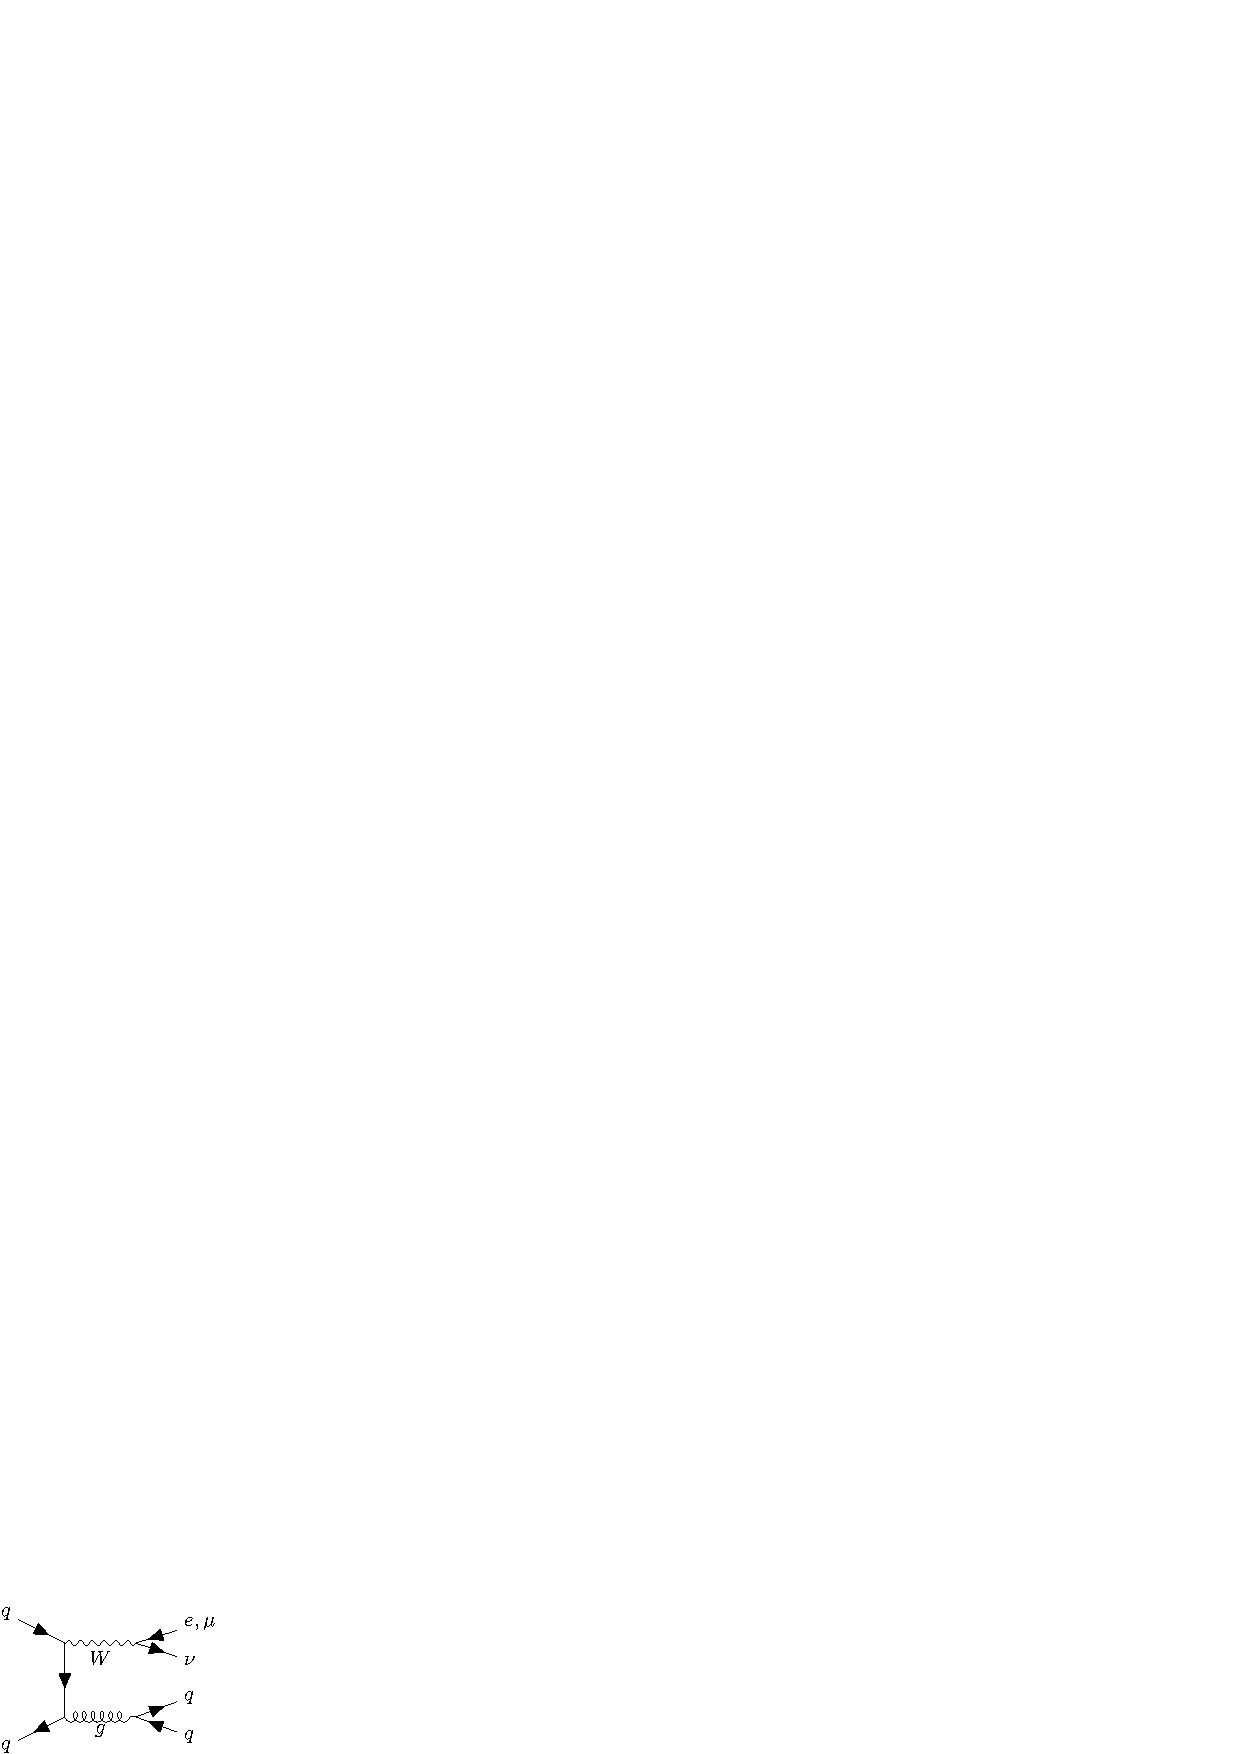
\includegraphics[width=0.95\textwidth]{figures/common/physics/wjets.pdf}
      \caption{\PW + jets}
    \end{subfigure}
    \hfill
    \begin{subfigure}{0.3\textwidth}
      \centering
      \includegraphics[width=0.95\textwidth]{figures/common/physics/ttbar.pdf}
      \caption{\ttbar production}
    \end{subfigure}
    \caption{Example Feynman graphs for the dominant background processes in searches for dark matter with heavy bosons.}
    \label{fig:common:analysis:backgroundgraphs}
\end{figure}

Other background processes include \HepProcess{\PW \PW}, \HepProcess{\PW \PZ}, and \HepProcess{\PZ \PZ} diboson production and production of single top quarks.

Finally, processes of pure strong interactions (referred to as multijet events) with poorly measured jet momenta give rise to fake \met and therefore can contribute as background. Although poor measurements of the jet momenta such that the fake \met is sufficient to pass the selection requirements occur infrequently, the overwhelming amount of multijet events at the LHC makes it necessary to adequately estimate this background.

The reconstructed \HepProcess{\Pp\Pp} collision events need to be categorised as either signal events or background events. To this end, the characteristic properties of the signal process are exploited to define discriminating variables, which can be used to separate signal and background events.

Event selection requirements based on the kinematic properties of reconstructed compound physics objects and on the event topology define a region enriched in signal processes, which is called the signal region (SR) and is characterised by a good sensitivity to the signal process.

The background contribution in the SR is estimated with samples of simulated events. As the simulation is subject to uncertainties, it is supplemented by data in dedicated control regions (CRs), which cover a similar phase-space as the SR but are enriched in the respective background processes. The SR and the CRs are defined by event selections which require different lepton multiplicities and therefore are disjoint.
The sharing of the background contributions among events with different lepton multiplicities depends on the \PW and \PZ boson branching ratios and the lepton reconstruction efficiencies, which are both well understood.
Therefore, the control region data enable reliable constraints of the background contributions in the SR, avoiding the sole reliance on theory predictions.

\Cref{fig:common:analysis:regions} illustrates the definition of SR and CRs in the searches for dark matter with heavy bosons. The 1 lepton CR allows constraining the \wjets and \ttbar processes in the SR, while the 2 lepton CR allows constraining the \zjets background in the SR using \HepProcess{\PZ \to \Pl \Pl} events.

\begin{figure}[htbp]
    \centering
    \includegraphics[width=0.75\textwidth]{figures/common/common_analysisregions.pdf}
    \caption{Illustration of the signal and control region definitions based on the lepton multiplicity. The control regions are enriched in specific background processes which populate the signal region and thereby allow for the estimation of these background contributions in the SR using data.}
    \label{fig:common:analysis:regions}
\end{figure}


\section{Data and simulated events}
\label{sec:common:data}
The \HepProcess{\Pp\Pp} collision data and the simulated physics processes are described in \Cref{sec:common:data:data} and \Cref{sec:common:data:mc}, respectively. The triggers used to select collision events are summarised in \Cref{sec:common:data:trigger}.

\subsection{Collision data}
\label{sec:common:data:data}
The searches for dark matter in association with heavy bosons are based on the LHC \HepProcess{\Pp\Pp} collision data recorded by the ATLAS detector in the years 2015--2018. Only collision events recorded during stable beam conditions with all detector subsystems fully operational are used for the physics analysis.

\Cref{fig:common:data:data} demonstrates the ATLAS data-taking performance during the Run-2 data-taking campaign, showing the total integrated luminosity and the mean number of interactions per bunch crossing.

\begin{figure}[htbp]
    \centering
    \begin{subfigure}{1.\textwidth}
      \centering
      \includegraphics[width=0.95\textwidth]{figures/common/intlumivstimeRun2DQall.pdf}
      \caption{Total integrated luminosity delivered by the LHC and recorded by the ATLAS detector during the Run-2 \HepProcess{\Pp\Pp} data-taking campaign. The fraction of the dataset satisfying the data quality requirements for physics analysis is indicated as ``Good for physics''.}
    \end{subfigure}
    \\
    \begin{subfigure}{1.\textwidth}
      \centering
      \includegraphics[width=0.9\textwidth]{figures/common/mu_2015_2018.pdf}
      \caption{Luminosity-weighted distribution of the mean number of interactions per bunch crossing for 2015, 2016, 2017, and 2018 \HepProcess{\Pp\Pp} collision data.}
    \end{subfigure}
    \caption{ATLAS data-taking performance during the Run-2 \HepProcess{\Pp\Pp} data-taking campaign. Figures reproduced from Ref.~\cite{DAPR-2018-01}.}
    \label{fig:common:data:data}
\end{figure}

In 2015, data with an integrated luminosity of \SI{3.2}{\per\femto\barn} was recorded with a data-taking efficiency of \SI{93}{\percent}, while in 2016 data corresponding to \SI{32.9}{\per\femto\barn} was recorded with a data-taking efficiency of \SI{92}{\percent}, resulting in a total integrated luminosity of \SI{36.1}{\per\femto\barn}.
The average number of interactions per bunch crossing \(\langle \mu \rangle\) was \num{13.7} during 2015 data-taking and \num{24.9} during 2016 data-taking.

The dataset recorded in 2017 with a data-taking efficiency of \SI{94}{\percent} corresponds to an integrated luminosity of \SI{43.8}{\per\femto\barn}.
The average number of interactions per bunch crossing \(\langle \mu \rangle\) was \num{37.8} during 2017 data-taking.
The 2015--2017 dataset corresponds to an integrated luminosity of \SI{79.8}{\per\femto\barn}

In 2018, data with an integrated luminosity of \SI{59.2}{\per\femto\barn} was recorded with a data-taking efficiency of \SI{93}{\percent}.
The average number of interactions per bunch crossing \(\langle \mu \rangle\) was \num{37.8} during 2018 data-taking.
The full Run-2 dataset recorded during the years 2015--2018 corresponds to an integrated luminosity of \SI{59.2}{\per\femto\barn}.


\subsection{Simulated event samples}
\label{sec:common:data:mc}
The signal and background contributions are estimated with Monte Carlo (MC) simulated event samples.
The simulated events are produced by MC event generators. The interactions of the generated particles with the detector are modelled with the \textsc{GEANT}~4~\cite{Agostinelli:2002hh} based ATLAS detector simulation~\cite{SOFT-2010-01}. The simulated collision events are reconstructed with the same trigger and reconstruction algorithms that are employed in collision data.

The simulated signal and background samples include the effect of in-time and out-of-time pile-up. This is achieved by overlaying inelastic \HepProcess{\Pp\Pp} collision events simulated using \PYTHIAV{8}, the \textsc{A3} tune~\cite{ATL-PHYS-PUB-2016-017}, and the \textsc{NNPDF23LO} PDF set~\cite{Ball:2012cx}. Simulated events are corrected using per-event weights to match the distribution of the number of interactions per bunch crossing as observed in data.

The \vjets backgrounds are simulated with the \SHERPAV{2.2.1} event generator~\cite{Bothmann2019}, with matrix elements computed at \NLO accuracy in QCD for up to two final-state partons and \LO accuracy in QCD for up to four final-state partons using Comix~\cite{Gleisberg:2008fv} and OpenLoops~\cite{Cascioli:2011va} with the \textsc{NNPDF30NNLO} PDF set~\cite{Ball2015}. The matrix elements are merged with the Sherpa parton shower~\cite{Schumann:2007mg} using the ME+PS@NLO prescription~\cite{Hoeche:2012yf}. The simulated events are normalised to an inclusive cross section with \NNLO precision in QCD~\cite{Melnikov:2006kv}.
Details of the generator configurations can be found in Ref.~\cite{ATL-PHYS-PUB-2017-006}.

Two sets of simulated samples for the top quark pair production and single top quark production backgrounds are available. The top quark mass was set to \SI{172.5}{\giga\electronvolt} in the event simulation.
In the first set, the simulation of top quark pair production involves matrix elements computed at \NLO accuracy in QCD with \POWHEGBOXV{2}~\cite{Alioli:2010xd} and the \textsc{CT10} PDF set~\cite{Lai2010}. The simulation of single top quark backgrounds in the \(s\)-channel and \(t\)-channels as well as the \(\PW t\) associated production are computed with \POWHEGBOXV{1}~\cite{Alioli:2010xd} using the fixed four-flavour PDF set \textsc{CT10f4}~\cite{Lai2010}. In all top-quark decays, the spin correlations were preserved using MadSpin~\cite{Artoisenet:2012st}. The parton shower and hadronisation is simulated using \PYTHIAV{6.428}~\cite{Sjostrand:2006za}, the \textsc{CTEQ6L1} PDF set~\cite{Pumplin:2002vw} and the corresponding \Perugia 2012 set~\cite{Skands:2010ak} of tuned parameters. The properties of \Pqb and \Pqc quark decays are described with \EVTGENV{1.2.0}~\cite{Lange:2001uf}.
In the second set, the simulation of both top quark pair production and single top quark production processes involves matrix elements computed accurately to \NLO QCD with \POWHEGBOXV{2}~\cite{Alioli:2010xd} using the \textsc{NNPDF30NLO} PDF set~\cite{Ball2015}, interfaced to the \PYTHIAV{8.230} parton shower and hadronisation model~\cite{Sjostrand:2014zea} using the \AFourteen set of tuned parameters ~\cite{ATL-PHYS-PUB-2014-021}.
The simulated events are normalised to a \NNLO QCD prediction for top quark pair production, including next-to-next-to-leading logarithmic corrections (\NLL) for soft gluon radiation~\cite{Czakon2013}, and to \NLO QCD predictions for single top quark processes~\cite{Stelzer1997,Stelzer1998,Smith1996,Kidonakis2013}.
Details on the configurations of both sets can be found in Ref.~\cite{ATL-PHYS-PUB-2018-009}.

Two sets of simulated samples for diboson processes are available, in which the diboson backgrounds are simulated with \SHERPA.
In the first set, the diboson production backgrounds with one weak gauge boson decaying leptonically and the other one decaying hadronically, are simulated with the \SHERPAV{2.1.1} event generator~\cite{Bothmann2019}. The matrix elements of the \HepProcess{\PZ\PZ} process were calculated in \NLO QCD accuracy for final states with at most one jet and in \LO QCD accuracy for final states with two or three jets, whereas those for \HepProcess{\PW\PZ} and \HepProcess{\PW\PW} processes were generated in \LO QCD for final states with up to three jets. In both cases, Comix~\cite{Gleisberg:2008fv} and OpenLoops~\cite{Cascioli:2011va} were used in conjunction with the \textsc{CT10} PDF set~\cite{Lai2010} and a dedicated tune provided by the Sherpa authors.
In the second set, all diboson background processes are simulated with the \SHERPAV{2.2.1} event generator~\cite{Bothmann2019}. The matrix elements of the process were calculated accurately to \NLO QCD for final states with at most one jet and accurate to \LO QCD for final states with two or three jets. The \textsc{NNPDF30NLO} PDF set~\cite{Ball2015} and a dedicated tune provided by the Sherpa authors were used.
Details of the generator configurations can be found in Ref.~\cite{ATL-PHYS-PUB-2017-005}.

Background processes from associated \VHbb production were generated with \POWHEGBOXV{2} interfaced to \PYTHIAV{8} using the \textsc{NNPDF30NLO} PDFs~\cite{Ball2015} and the AZNLO tune~\cite{STDM-2012-23}. Both the quark-induced \HepProcess{\PW\PHiggs} and \HepProcess{\PZ\PHiggs} production, as well as the gluon-induced \HepProcess{\PZ \PHiggs} production are considered. The event samples are normalised to the best available theoretical predictions at \NNLO accuracy in QCD and \NLO accuracy in electroweak corrections~\cite{CERN2017}.

Multijet background processes are typically estimated using data-driven methods, as their MC simulation is computationally costly. However, for the development and optimisation of these background estimation methods, a MC simulated sample is used. This sample is generated using the \PYTHIAV{8.230} event generator~\cite{Bothmann2019}, incorporating LO matrix elements and a model describing parton shower and hadronisation, both computed using the \textsc{NNPDF23LO} PDF set~\cite{Ball:2012cx}. The \AFourteen set of tuned parameters~\cite{ATL-PHYS-PUB-2014-021} is used.

A summary of all simulated background samples is provided in \Cref{tab:common:data:mc:generators}.

\begin{table}[htbp]
\caption{List of the simulated background processes in searches for dark matter with heavy vector bosons with the event generators, PDF sets, parton shower models, set of tuned parameters (``tunes''), and the accuracy in QCD of the modelling and the cross-section.}
\label{tab:common:data:mc:generators}
\centering
\resizebox{1.\textwidth}{!}{%
\begin{tabular}{l l l l l l}
\toprule
Process & Generator & Parton shower & PDF & Tune & Accuracy in QCD          \\
        &           &               &     &      & (modelling /             \\
        &           &               &     &      & inclusive cross-section) \\
\midrule
\textbf{\(V\) + jets} & & & & & \\
\Wjets & \SHERPAV{2.2.1} & \SHERPAV{2.2.1} & \textsc{NNPDF30NNLO} & \SHERPA-tune & \NLO / \NNLO \\
\Zjets & \SHERPAV{2.2.1} & \SHERPAV{2.2.1} & \textsc{NNPDF30NNLO} & \SHERPA-tune & \NLO / \NNLO \\
\midrule
\textbf{Top quark} & & & & & \\
\ttbar               & \POWHEGBOXV{2} & \PYTHIAV{6.428} & \textsc{CT10}       & \Perugia 2012 & \NLO / \NNLO + \NLL \\
                     & \POWHEGBOXV{2} & \PYTHIAV{8.230} & \textsc{NNPDF30NLO} & \AFourteen    & \NLO / \NNLO + \NLL \\
\Pqt (\(s\)-channel) & \POWHEGBOXV{1} & \PYTHIAV{6.428} & \textsc{CT10}       & \Perugia 2012 & \NLO / \NLO \\
                     & \POWHEGBOXV{2} & \PYTHIAV{8.230} & \textsc{NNPDF30NLO} & \AFourteen    & \NLO / \NLO \\
\Pqt (\(t\)-channel) & \POWHEGBOXV{1} & \PYTHIAV{6.428} & \textsc{CT10}       & \Perugia 2012 & \NLO / \NLO \\
                     & \POWHEGBOXV{2} & \PYTHIAV{8.230} & \textsc{NNPDF30NLO} & \AFourteen    & \NLO / \NLO \\
\Pqt (\(\PW t\))     & \POWHEGBOXV{1} & \PYTHIAV{6.428} & \textsc{CT10}       & \Perugia 2012 & \NLO / \NLO \\
                     & \POWHEGBOXV{2} & \PYTHIAV{8.230} & \textsc{NNPDF30NLO} & \AFourteen    & \NLO / \NLO \\
\midrule
\textbf{Diboson} & & & & & \\
\HepProcess{\PW\PW} & \SHERPAV{2.1.1} & \SHERPAV{2.1.1} & \textsc{CT10}       & \SHERPA-tune  & \NLO / \NLO \\
                    & \SHERPAV{2.2.1} & \SHERPAV{2.2.1} & \textsc{NNPDF30NLO} & \SHERPA-tune  & \NLO / \NLO \\
\HepProcess{\PW\PZ} & \SHERPAV{2.1.1} & \SHERPAV{2.1.1} & \textsc{CT10}       & \SHERPA-tune  & \NLO / \NLO \\
                    & \SHERPAV{2.2.1} & \SHERPAV{2.2.1} & \textsc{NNPDF30NLO} & \SHERPA-tune  & \NLO / \NLO \\
\HepProcess{\PZ\PZ} & \SHERPAV{2.1.1} & \SHERPAV{2.1.1} & \textsc{CT10}       & \SHERPA-tune  & \NLO / \NLO \\
                    & \SHERPAV{2.2.1} & \SHERPAV{2.2.1} & \textsc{NNPDF30NLO} & \SHERPA-tune  & \NLO / \NLO \\
\midrule
\VHbb               & \POWHEGBOXV{2}  & \PYTHIAV{8.212} & \textsc{NNPDF30NLO} & \AZNLO        & \NLO / \NNLO \\
Multijet            & \PYTHIAV{8.230} & \PYTHIAV{8.230} & \textsc{NNPDF23LO}  & \AFourteen    & \LO  / \LO   \\
\bottomrule
\end{tabular}%
}
\end{table}


\subsection{Triggers}
\label{sec:common:data:trigger}
The events are selected by a combination of trigger algorithms, which are based on the two-staged trigger system comprised by the L1 trigger and the HLT (c.f. \Cref{sec:experiment:ATLAS:trigger}). Two types of trigger algorithms are employed in the searches for dark matter with heavy bosons.
\begin{itemize}
  \item \met triggers are used to select events for the 0 lepton SR and for the 1 muon CR.
  \item Single lepton (\Pe / \Pgm) triggers are used to select events for the 2 lepton CR.
\end{itemize}
The use of \met triggers for the 1 muon CR is enabled by restricting the corresponding lepton selection to muons, as the particular computation of \met on trigger level takes into account only information provided by the calorimeters. Muons traversing the calorimeter only deposit a negligible amount of their energy, therefore they contribute to \met on trigger level.

The instantaneous luminosity increases with data-taking periods, therefore the trigger thresholds have to be adapted accordingly.
The triggers are defined by the L1 and HLT algorithms (c.f. \Cref{sec:experiment:ATLAS:trigger}) and corresponding thresholds, which are encoded in their names. For instance, the \textsc{HLT\_xe90\_mht\_L1XE50} trigger requires the L1 \met to exceed \SI{50}{\giga\electronvolt} and the \met reconstructed by the HLT algorithm to exceed \SI{90}{\giga\electronvolt}. Similarly, the \textsc{HLT\_mu50} trigger requires that an HLT algorithm detects a muon with \(\pt > \SI{50}{\giga\electronvolt}\).

The \met triggers are based different algorithms~\cite{TRIG-2019-01}. The \met trigger used in 2015 data-taking is based on an the \textsc{cell} algorithm, which calculates \met on trigger level using towers of calorimeter cells. The \textsc{mht} algorithm employed in 2016 data-taking calculates the \met on trigger level as the negative \pt vector sum of all jets with \(\pt > \SI{7}{\giga\electronvolt}\) before JES calibration, which were reconstructed using the \antikt algorithm with radius parameter \(R=0.4\) from calorimeter topological clusters.
The \textsc{pufit} algorithm employed in 2017--2018 data-taking calculates the \met from \(\eta\)-\(\varphi\) patches that correspond approximately the size of jets with radius parameter \(R=0.4\), which are created from calorimeter topological clusters and are corrected for pile-up contributions by a \(\chi^2\)-fit.
The \met trigger thresholds range from \SI{70}{\giga\electronvolt} to \SI{110}{\giga\electronvolt} during the 2015--2018 data-taking periods.

The single-lepton triggers impose requirements on electrons and muons identified by the L1 and HLT algorithms. The L1 requirement on the electron \(E_{\text{T}}\) or muon \pt imposes a looser threshold than that of the HLT algorithms. The better resolution of the HLT algorithms allows setting tighter cuts, ranging from \SIrange{24}{300}{\giga\electronvolt} for electrons and \SIrange{20}{50}{\giga\electronvolt} for muons. Additional requirements on the lepton identification (\textsc{lhloose}, \textsc{lhmedium}, \textsc{lhtight}), on the isolation criteria (\textsc{iloose}, \textsc{imedium}), and on the transverse impact parameter (\textsc{nod0}) are defined, which improve the trigger selectivity. A combination of lepton triggers with low-\pt thresholds requiring additional isolation criteria and triggers with high-\pt thresholds but no further requirements is used to preserve the trigger efficiency for high-\pt leptons.

The trigger efficiency is defined as
\begin{align}
    \varepsilon = \frac{N(\text{trigger} | \mathcal{S}_{i})}{N(\mathcal{S}_{i})},
\end{align}
where \(N(\mathcal{S}_{i})\) denotes the number of events satisfying the selection \(\mathcal{S}_{i}\) and \(N(\text{trigger} | \mathcal{S}_{i})\) denotes the number of events that also satisfies the trigger requirement.

The \met trigger efficiency for different years of the Run-2 data-taking is shown in \Cref{fig:common:data:trigger:mettriggerefficiency}.

\begin{figure}[htbp]
  \centering
  \includegraphics[width=0.95\textwidth]{figures/common/met_trigger_efficiency.pdf}
  \caption{Combined L1 and HLT efficiency of the \met triggers with lowest threshold used in each year of data-taking. The \met trigger efficiency is measured in data using \HepProcess{\PZ \to \Pgm\Pgm} events and is shown as a function of the \PZ boson transverse momentum \(\pt^{\mu\mu}\). Figure reproduced from Ref.~\cite{TRIG-2019-01}.}
  \label{fig:common:data:trigger:mettriggerefficiency}
\end{figure}

The reduced efficiency for \(\met < \SI{200}{\giga\electronvolt}\) is due to the limited detector resolution, which results in differences between \met reconstructed on trigger level and the offline \met.

In the searches for dark matter with heavy bosons, the \met trigger threshold dictates the lowest possible selection requirement on \met. As these searches investigate events with \(\met > \SI{150}{\giga\electronvolt}\), the trigger (in)efficiency needs to be studied in data and MC to derive corrections for potential discrepancies between simulation and data.

The \met trigger calibration is performed in events passing single-muon triggers, since the calculation of \met on trigger level does not involve muons. The \met trigger efficiency is measured as a function of \metnomu, which is calculated by excluding muons from the \met reconstruction. It is parametrised in the region \(\SI{120}{\giga\electronvolt} < \metnomu < \SI{300}{\giga\electronvolt}\) by the function
\begin{align}
    f(\metnomu) = \frac{1}{2} \left[1 + \text{Erf}\left(\frac{\metnomu - a}{\sqrt{2} b}\right)\right],
    \label{eq:common:trigger:met:calibration}
\end{align}
where \(\text{Erf}(x)\) denotes the error function and \(a,b \in \mathbb{R}\) are free parameters in the fit.

The \met trigger efficiency corrections for simulated events are obtained as the ratio of the \met trigger efficiency measured in data and in simulated samples of background processes. These corrections can depend on the multiplicity of \bjets in the event due to the different calorimeter responses for light-flavour and heavy-flavour jets.
While the nominal \met trigger efficiency corrections are derived from a selection inclusive in the \bjet multiplicity, the associated systematic uncertainties are evaluated by comparing the nominal scale-factors obtained from the inclusive selection with scale-factors obtained from a selection requiring the presence of at least one \btagged jet.
The total uncertainty on the \met trigger calibration additionally takes into account the \(1\sigma\) confidence interval of the fit based on \Cref{eq:common:trigger:met:calibration}.

A similar calibration is performed for the single lepton triggers~\cite{TRIG-2018-01,TRIG-2018-05}. The object definitions of leptons are designed to ensure that the lepton triggers are fully efficient.


\section{Object definitions in searches for dark matter produced in association with heavy bosons}
\label{sec:common:objects}
The physical objects used for the event selection and the reconstruction of the kinematic properties of collision events in the searches for dark matter with heavy bosons are introduced in the following. Various object definitions with different requirements on kinematic properties, identification and isolation criteria are employed to accommodate the competing needs concerning purity and reconstruction efficiency.

Three types of jets are considered in the physics object definitions and in the definition of selection criteria to enhance the sensitivity of the searches. The small-radius jets and large-radius jets are used for reconstructing the hadronic decays of heavy bosons, while the track jets supplement the large-radius jets with \btagging information.

The \textbf{small-radius jets} are divided into two categories based on their pseudorapidity.
The jets with \(\abs{\eta} < 2.5\) are referred to as central jets. Jets originating from pile-up are suppressed by requiring the central jets with \(\pt < \SI{60}{\giga\electronvolt}\) and \(\abs{\eta} < 2.4\) to be associated with the primary vertex. Therefore, these jets are required to pass the Jet Vertex Tagger (JVT) requirements with a JVT score of \(\text{JVT} > 0.59\). Residual differences in the JVT score evaluation between data and simulation are taken into account by applying scale-factors to the weight of MC simulated events.
The central jets originating from \bquarks are referred to as \bjets. They are identified using the MV2 \btagging algorithm with fixed-cut efficiency operating points corresponding to \SI{70}{\percent} and \SI{77}{\percent} \btagging efficiency.
The small-radius jets with \(2.5 < \abs{\eta} < 4.5\) and \(\pt > \SI{30}{\giga\electronvolt}\) are referred to as forward jets. They are used only in selection requirements to suppress background processes. In particular, the requirements to reject multijet background events with fake \met use the information provided by these jets.
The common definitions of small-radius jets are summarised in \Cref{tab:common:objects:jets:smallr}.

\begin{table}[htbp]
\caption{Common definitions of small-radius jets.}
\label{tab:common:objects:jets:smallr}
\centering
\resizebox{1.\textwidth}{!}{%
\begin{tabular}{l lll}
\toprule
& Central jets & \bjets & Forward jets \\
\midrule
Jet algorithm & \antikt & \antikt & \antikt\\
\(R\)-parameter & \num{0.4} & \num{0.4} & \num{0.4}\\
Input constituents & EMTopo & EMTopo & EMTopo \\
Pseudorapidity range & \(\abs{\eta} < 2.5\) & \(\abs{\eta} < 2.5\) & \(2.5 < \abs{\eta} < 4.5\) \\
Transverse momentum  & \(\pt > \SI{20}{\giga\electronvolt}\) & \(\pt > \SI{20}{\giga\electronvolt}\) & \(\pt > \SI{30}{\giga\electronvolt}\) \\
JVT & \multicolumn{2}{c}{\(> 0.59\) for \(\pt < \SI{60}{\giga\electronvolt}\), \(\abs{\eta} < 2.4\)} & no\\
\(b\)-tagging & no & MV2 (\SI{70}{\percent} / \SI{77}{\percent} efficiency) & no \\
\bottomrule
\end{tabular} %
}
\end{table}

The \textbf{large-radius jets} are used to identify weak vector bosons with large Lorentz boost. The trimming algorithm (c.f. \Cref{sec:methods:event-reconstruction:jets:larger}) is applied to remove energy deposits from pile-up with radius parameter \(R_{\text{sub}} = 0.2\) and momentum fraction \(f_{\text{cut}} = 0.05\). The requirements on the kinematic properties \(\pt > \SI{100}{\giga\electronvolt}\) and \(\abs{\eta} < 2.0\) ensure the reconstruction of high-\pt jets in the central region of the detector with good overlap between the ID and the calorimeters.

The \textbf{track jets} are used to identify the flavour content of the large-radius jets. In the scope of this dissertation, both track jet definitions with a fixed radius parameter \(R=0.2\) (FR) and a variable radius parameter (VR) are considered.
Both FR and VR track jets are required to satisfy \(\pt > \SI{10}{\giga\electronvolt}\), \(\abs{\eta} < 2.5\), and are required to have at least two constituent tracks. The VR track jets must satisfy an additional requirement on the separation of individual VR track jets \(\Delta R > 0.02\) to rejects events with concentric pairs of VR track jets, which are problematic for a stable \btagging performance.
The \btagged track jets are identified using the MV2 \btagging algorithm with fixed-cut efficiency of either \SI{70}{\percent} or \SI{77}{\percent} \btagging efficiency. The \btagging performance of track jets in simulations is corrected to that in data by a calibration based on a combinatorial likelihood approach in a sample of \ttbar events~\cite{PERF-2016-05}.
The common definitions of large-radius jets and track jets are summarised in \Cref{tab:common:objects:jets:boosted}.

\begin{table}[h]
\caption{Common definitions of jets used for boosted heavy boson reconstruction}
\label{tab:common:objects:jets:boosted}
\resizebox{1.\textwidth}{!}{%
\begin{tabular}{l lll}
\toprule
 & Large-radius jets & VR track jets & FR track jets \\
\midrule
Jet algorithm & \antikt & \antikt & \antikt\\
\(R\)-parameter & \num{1.0} & \(R_{\text{eff}}\) & \num{0.2} \\
Grooming algorithm & trimming & no & no \\
\(R_{\text{sub}}\) & \num{0.2} & no & no \\
\(f_{cut}\) & \num{0.05} & no & no \\
Input constituents & LCTopo  & tracks & tracks \\
Pseudorapidity range & \(\abs{\eta} < 2.0\) & \(\abs{\eta} < 2.5\) & \(\abs{\eta} < 2.5\)  \\
Transverse momentum & \(\pt > \SI{100}{\giga\electronvolt}\) & \(\pt > \SI{10}{\giga\electronvolt}\) & \(\pt > \SI{10}{\giga\electronvolt}\) \\
\btagging & no & MV2 (\SI{77}{\percent} efficiency) & MV2 (\SI{70}{\percent} / \SI{77}{\percent} efficiency) \\
\bottomrule
\end{tabular}%
}
\end{table}

Two types of \textbf{electron} definitions are considered. Baseline electron candidates are used to define vetoes on electrons in the event selection. They are reconstructed using the \textsc{Loose} ID OP in conjunction with the \textsc{LooseTrackOnly} isolation OP and have to satisfy the kinematic requirements \(\pt > \SI{7}{\giga\electronvolt}\) and \(\abs{\eta} < 2.47\).
Signal electron candidates are used to select pairs of electrons. They are required to satisfy stricter requirements on their transverse energy. In searches considering 2015--2016 data, \(E_{\text{T}} > \SI{25}{\giga\electronvolt}\) is required, while the increased single electron trigger thresholds in 2017--2018 necessitate signal electron candidates with \(E_{\text{T}} > \SI{27}{\giga\electronvolt}\) in order to ensure the full efficiency of the employed single electron trigger.
Both baseline and signal electron candidates have to satisfy requirements on the impact parameters \(\abs{d_{0}} / \sigma(d_{0}) < 5\) and \(\abs{z_{0}} \sin \theta < \SI{0.5}{\milli\meter}\).
The definitions of baseline and signal electron candidates are summarised in \Cref{tab:common:objects:electrons}.

\begin{table}[htbp]
\caption{Common definitions of electron candidates.}
\label{tab:common:objects:electrons}
\centering
\begin{tabular}[ht]{l ll}
  \toprule
  & Baseline & Signal \\
  \midrule
  Pseudorapidity range & \(\abs{\eta} < 2.47\) & \(\abs{\eta} < 2.47\) \\
  Transverse energy & \(E_{\text{T}} > \SI{7}{\giga\electronvolt}\) & \(E_{\text{T}} > \SI{25}{\giga\electronvolt} / \SI{27}{\giga\electronvolt}\) \\
  Identification & Loose & Medium \\
  Isolation & LooseTrackOnly & LooseTrackOnly \\
  Track to vertex & \(\abs{d_{0}} / \sigma(d_{0}) < 5\) & \(\abs{d_{0}} / \sigma(d_{0}) < 5\) \\
  association & \(\abs{z_{0}} \sin \theta < \SI{0.5}{\milli\meter}\) & \(\abs{z_{0}} \sin \theta < \SI{0.5}{\milli\meter}\) \\
  \bottomrule
 \end{tabular}
\end{table}

Three types of \textbf{muon} definitions are considered. Baseline muon candidates are used to define the vetoes on muons in the event selection. They are reconstructed using the \textsc{Loose} ID OP in conjunction with the \textsc{LooseTrackOnly} isolation OP and have to satisfy the kinematic requirements \(\pt > \SI{7}{\giga\electronvolt}\) and \(\abs{\eta} < 2.7\).
Signal muon candidates are used to select pairs of muons. They are required to satisfy stricter kinematic requirements \(\pt > \SI{25}{\giga\electronvolt}\) and \(\abs{\eta} < 2.5\).
Tight signal muon candidates are used to select individual muons. They are reconstructed using the \textsc{Medium} ID OP in conjunction with the \textsc{TightTrackOnly} isolation OP and otherwise satisfy the signal muon candidate kinematic requirements.
Baseline, signal, and tight signal muon candidates have to satisfy requirements on the impact parameters \(\abs{d_{0}} / \sigma(d_{0}) < 3\) and \(\abs{z_{0}} \sin \theta < \SI{0.5}{\milli\meter}\).
The definitions of baseline, signal, and tight signal muons are summarised in \Cref{tab:common:objects:muons}.

\begin{table}[htbp]
\caption{Common definitions of muon candidates.}
\label{tab:common:objects:muons}
\centering
\resizebox{1.\textwidth}{!}{%
\begin{tabular}[ht]{l lll}
  \toprule
  & Baseline & Signal & Tight signal \\
  \midrule
  Pseudorapidity range & \(\abs{\eta} < 2.7\) & \(\abs{\eta} < 2.5\) & \(\abs{\eta} < 2.5\) \\
  Transverse momentum & \(\pt > \SI{7}{\giga\electronvolt}\) & \(\pt > \SI{25}{\giga\electronvolt}\) & \(\pt > \SI{25}{\giga\electronvolt}\) \\
  Identification & Loose & Loose & Medium \\
  Isolation & LooseTrackOnly & LooseTrackOnly & TightTrackOnly \\
  Track to vertex & \(\abs{d_{0}} / \sigma(d_{0}) < 3\) & \(\abs{d_{0}} / \sigma(d_{0}) < 3\) & \(\abs{d_{0}} / \sigma(d_{0}) < 3\) \\
  association & \(\abs{z_{0}} \sin \theta < \SI{0.5}{\milli\meter}\) & \(\abs{z_{0}} \sin \theta < \SI{0.5}{\milli\meter}\) & \(\abs{z_{0}} \sin \theta < \SI{0.5}{\milli\meter}\) \\
  \bottomrule
 \end{tabular}%
 }
\end{table}

Hadronically decaying \textbf{tau leptons} are identified using small-radius jets. Baseline tau lepton candidates can be used to veto events containing tau leptons, as the signature targeted by the searches with heavy bosons does not include these.
Baseline tau lepton candidates are required to satisfy \(\pt > \SI{20}{\giga\electronvolt}\) and \(\abs{\eta} < 2.5\), excluding the region \(1.37 < \abs{\eta} < 1.52\) because of a gap in the instrumentation of the calorimeters. The topology of tau decays is exploited to avoid the misidentification of jets, electrons, or muons as tau leptons, by using a set of Boosted Decision Trees (BDTs) to classify the tracks associated with the jet and requiring the presence of either one or three core tracks.
The object definition for baseline tau lepton candidates is summarised in \Cref{tab:common:objects:taus}.

\begin{table}[htbp]
\caption{Common definition of tau lepton candidates.}
\label{tab:common:objects:taus}
\centering
\begin{tabular}[ht]{l l}
  \toprule
  & Baseline \\
  \midrule
  Pseudorapidity range & \(\abs{\eta} < 2.5\), excluding \(1.37 < \abs{\eta} < 1.52\) \\
  Transverse momentum & \(\pt > \SI{20}{\giga\electronvolt}\) \\
  Track selection & 1 or 3 tracks \\
  \bottomrule
 \end{tabular}
\end{table}